\documentclass{article}

\usepackage{url}
\usepackage{nicefrac}
\usepackage{amssymb,amsfonts,amsmath,amsthm}
\usepackage{mathtools}
\usepackage{adjustbox}
\usepackage{bm}
\usepackage{bbold}
\usepackage[margin=60pt]{geometry}
\pdfinclusioncopyfonts=1

\usepackage{xcolor}
\definecolor{RED}{HTML}{EB6231}
\definecolor{YELLOW}{HTML}{E29D26}
\definecolor{BLUE}{HTML}{5D80B4}
\definecolor{LIGHTGREEN}{HTML}{6ABD9B}
\definecolor{GREEN}{HTML}{8FB03E}
\definecolor{PURPLE}{HTML}{BE1E2D}
\definecolor{BROWN}{HTML}{A97C50}
\definecolor{PINK}{HTML}{DA1C5C}

\newcommand{\specialcell}[2][c]{%
	\begin{tabular}[#1]{@{}c@{}}#2\end{tabular}}

\newcommand{\der}{\mathrm{d}}
\newcommand{\e}{\mathrm{e}}
\newcommand{\dnds}{dN/dS}
\newcommand{\indice}{l}
\newcommand{\indiceexp}{^{(\indice)}}
\newcommand{\angstrom}{\text{\normalfont\AA}}

% Time, effective population size and mutation rate.
\newcommand{\Ne}{N_{\mathrm{e}}}
\newcommand{\Nsite}{S}
\newcommand{\site}{\text{s}}
% DNA

\newcommand{\ci}{{i}}
\newcommand{\cj}{{j}}
\newcommand{\itoj}{\ci, \cj}
\newcommand{\nucitoj}{\ci \rightarrow \cj}
\newcommand{\submatrix}{Q}


\newcommand{\phenoDiv}{S}
\newcommand{\phenoGeo}{\bm{P}}
\newcommand{\phenoFold}{\Delta G}

\begin{document}

\part*{Simulations}

\section{Simulation with independent fitness profiles}

Overall, the protein phenotype is computed as the sum of site-specific selection coefficient, obtained by accessing the amino-acid present at each site of the protein.
From a DNA sequence $\mathbb{S}^t$ after $t$ substitutions, the protein's phenotype is given by:
\begin{equation}
\phenoGeo\left(\mathbb{S}^{t}\right) = \sum_{1 \leq \site \leq \Nsite} \phenoGeo_{\site} \left(\mathbb{S}^t(\site) \right),
\end{equation}
where $\phenoGeo_{\site}$ is the genotype-phenotype map at site $\site$.\\

And the fitness of $\mathbb{S}^t$ is : 
\begin{equation}
w\left( \phenoGeo\left(\mathbb{S}^{t}\right) \right) = e^{-\alpha \left| \phenoGeo\left(\mathbb{S}^{t}\right) \right|^{\beta}},
\end{equation}
where strength ($\alpha > 0$) and epistasis ($\beta$) are parameters of the fitness function.

The Malthusian fitness selection coefficients $f$ at site $\site$, are obtained by taking the logarithm of the fitness profile assigned to this site:
\begin{equation}
\label{eq:sitefitness}
f = \ln \left( g \right)
\end{equation}

\begin{center}
	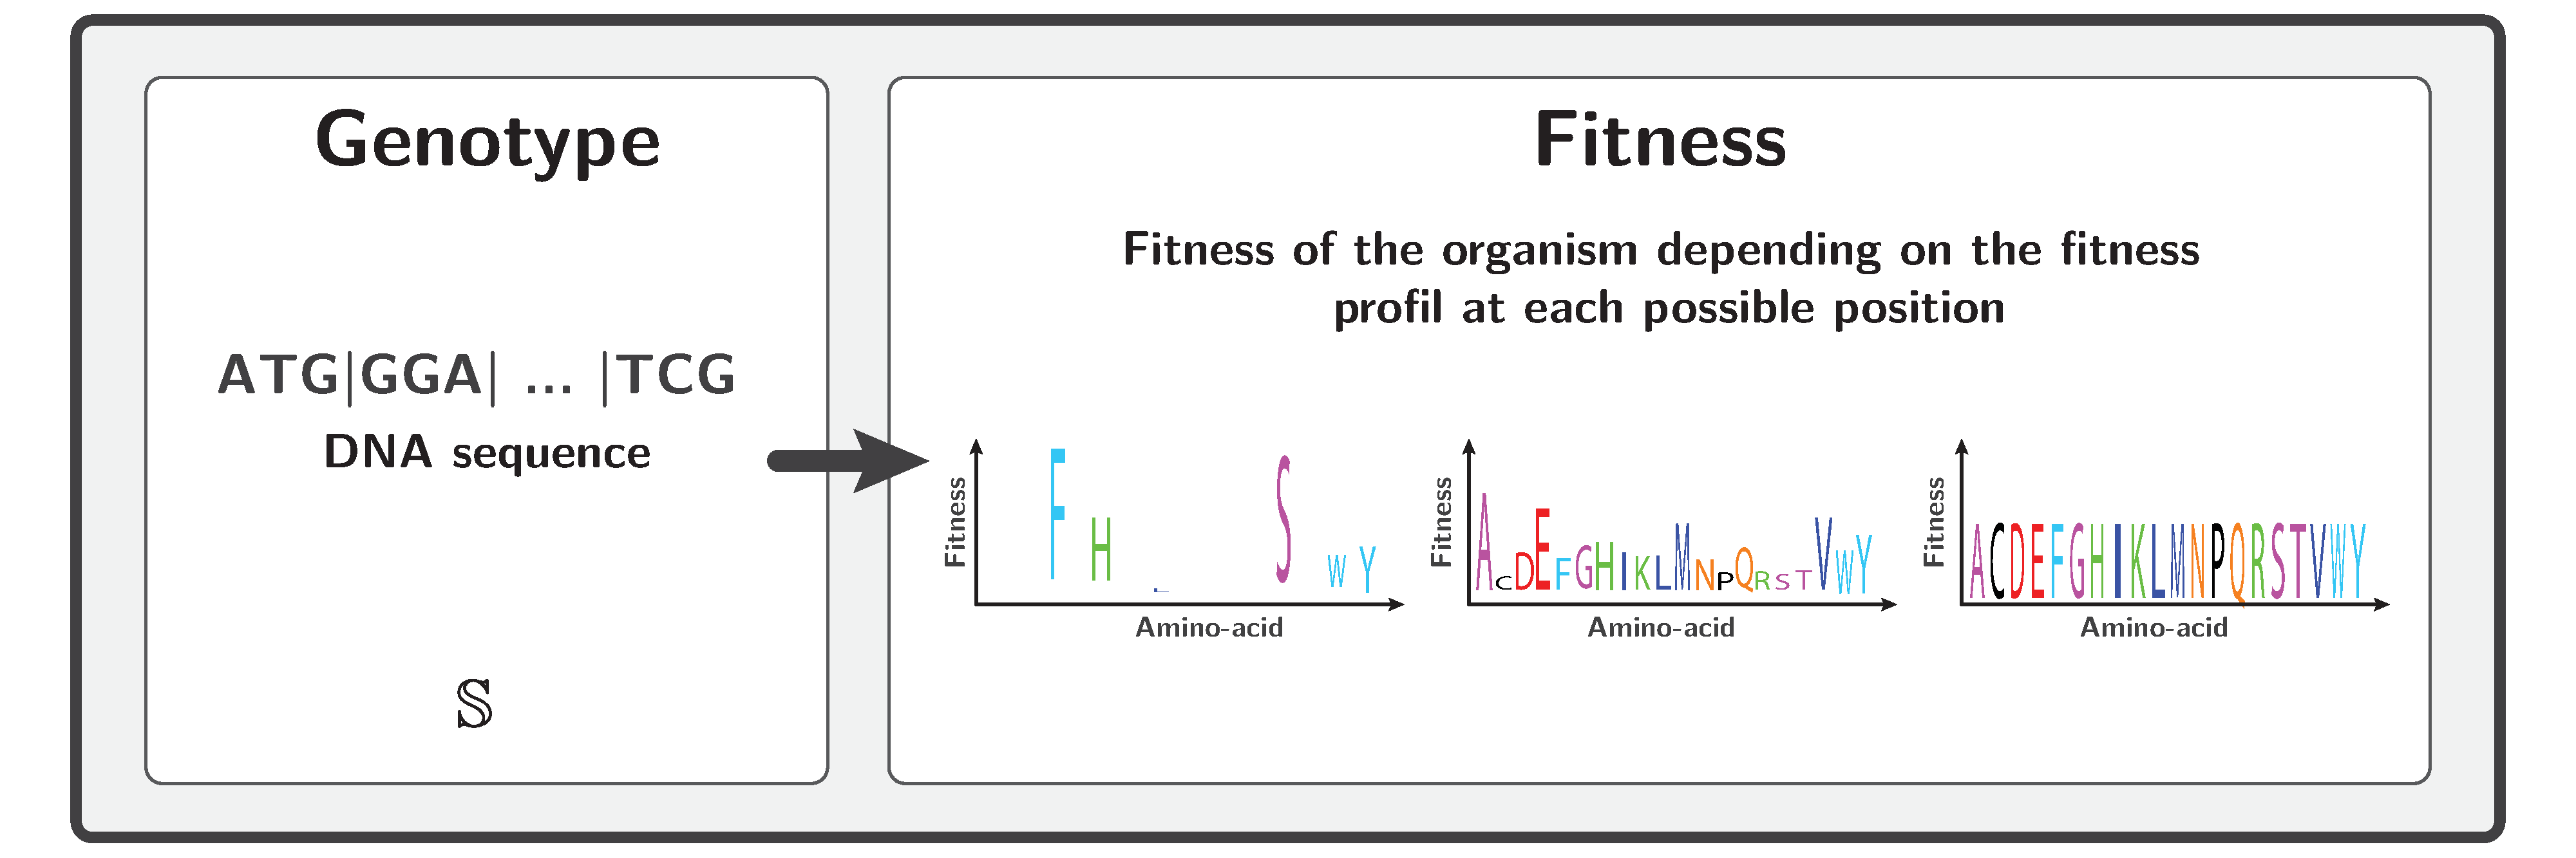
\includegraphics[width=165mm] {artworks/ModelSimuDiv.pdf}
\end{center}

For each possible mutant ($t+1$ substitutions), we compute $\phenoGeo\left(\mathbb{S}^{t+1}\right)$ from the updated sequence $\mathbb{S}^{t+1}$, and subsequently the selection coefficient of the mutant:
\begin{equation}
s \left( \mathbb{S}^{t},\mathbb{S}^{t+1}\right) = \ln 
\end{equation}
The next change in the protein coding DNA and the time to next the event is chosen using Gillespie algorithm, according to the rates of substitution between codons:
\begin{equation}
{\submatrix_{\itoj}} = \mu_{\itoj} \dfrac{4 \Ne s \left( \mathbb{S}^{t},\mathbb{S}^{t+1}\right)}{{1 - \e^{-4 \Ne \left( \mathbb{S}^{t},\mathbb{S}^{t+1}\right)} }}, 
\end{equation}
where ${\submatrix_{\itoj}} = \mu_{\itoj}$ in the case of synonymous substitutions.

\section{Simulation in Wright-Fisher context}

The evolutionary dynamics was formalized as a Wright-Fisher model with mutation, selection and drift. The population is assumed to be panmictic, with constant size $N_e$ and with non-overlapping generations. 

The sites mutate at rate $u$ per generation. Each non-synonymous mutation produces a new functional PRDM9 variant


\begin{center}
	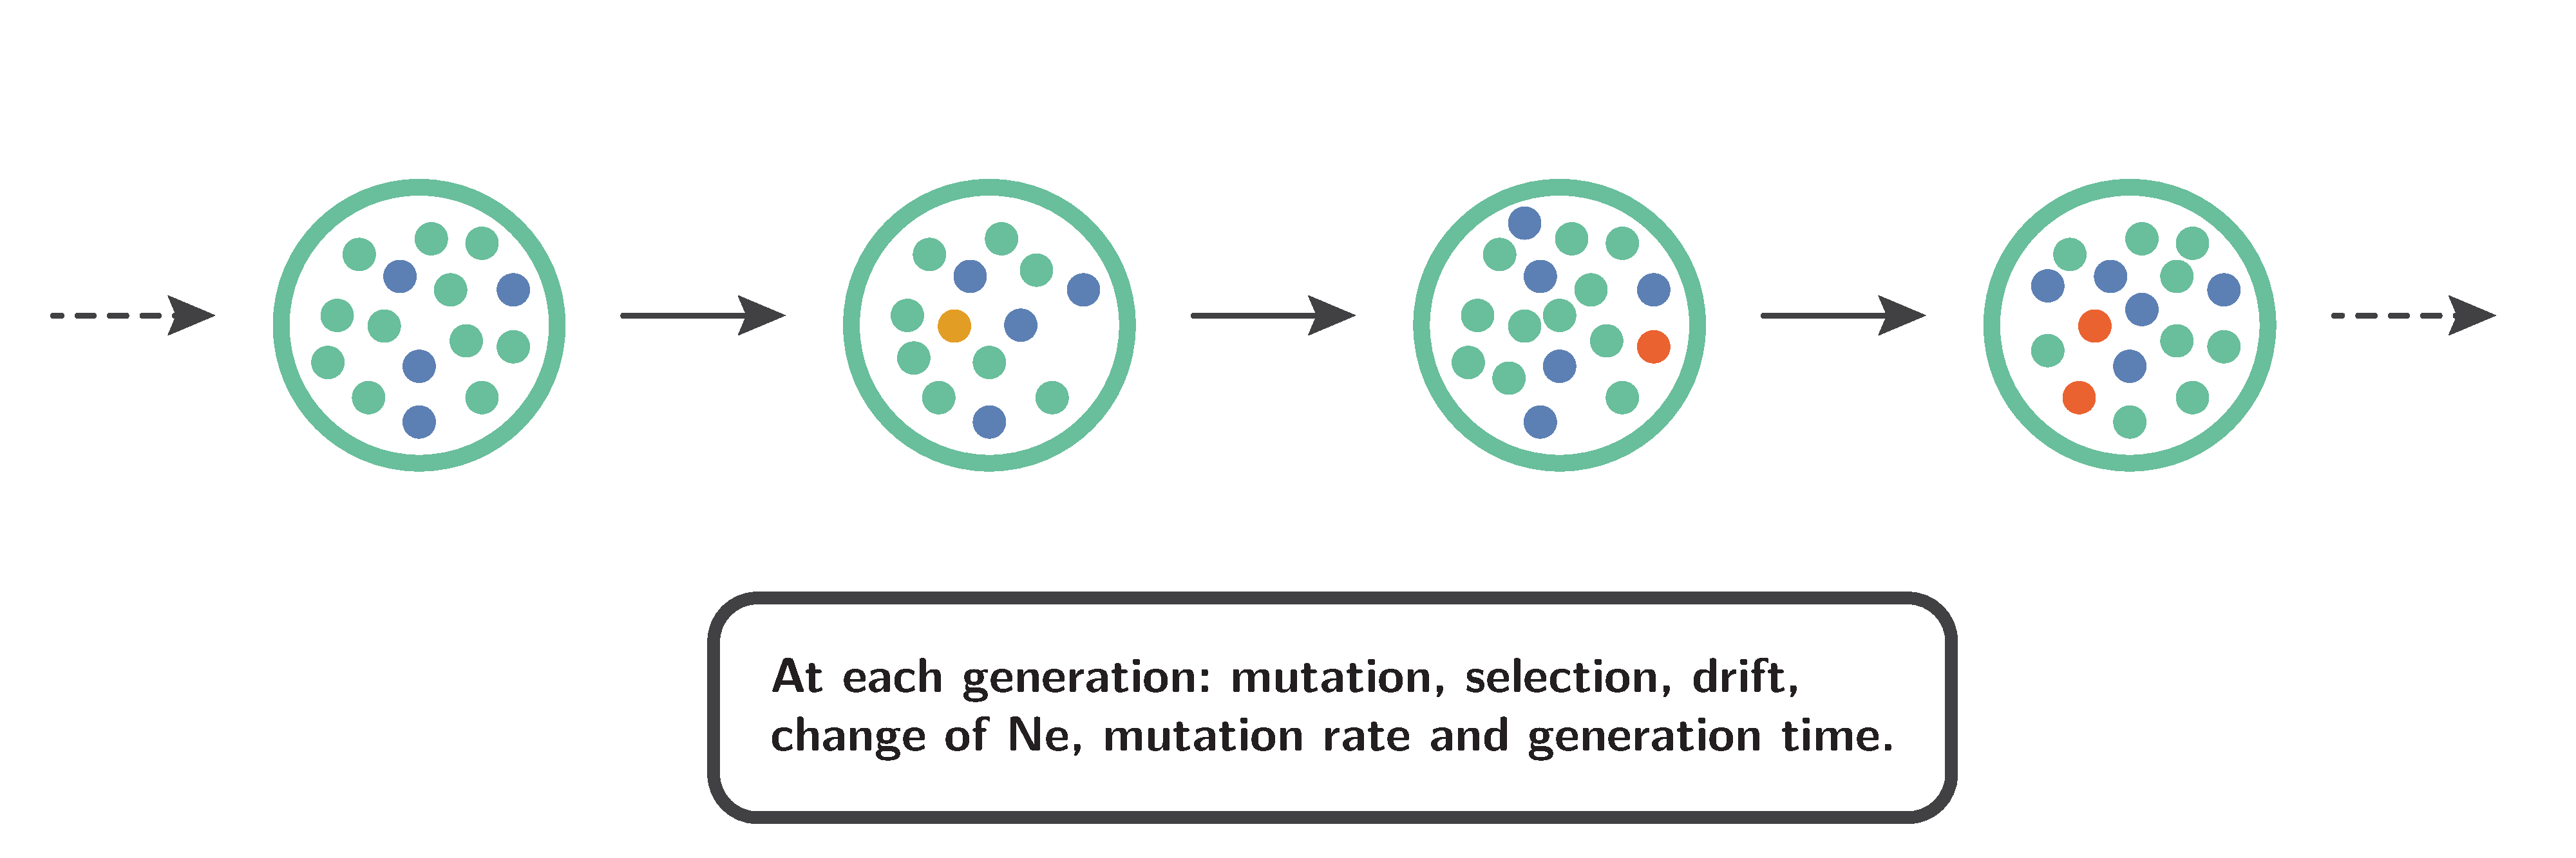
\includegraphics[width=165mm] {artworks/ModelSimuPoly.pdf}
\end{center}

\section{Simulation with Fisher geometric landscape}

We simulated substitutions in a protein using an adaptation of Fisher's geometric landscape.
In the original context, the phenotype is a vector ($\phenoGeo$) in a multidimensional space, where the number of dimensions is often termed complexity.
From a phenotype, the fitness is a monotonously decreasing function of the phenotype distance to $0$.
The exact functional phenotype-fitness map depend on $2$ external parameters controlling for strength ($\alpha$) and epistasis ($\beta$).
If the phenotype-fitness map is explicit, the genotype-phenotype map is more pervasive.
Mutations are seen has displacement of the phenotype in the multidimensional space.
Beneficial mutations are moving the phenotype closer to $0$, whereas deleterious mutations are moving the phenotype further away.
In such original context, the distribution of mutational effects is not dependent on the current genotype, but this can be relaxed using a genotype-phenotype map.\\

In a protein context, the genotype-phenotype map can be defined by assigning to each of the $20$ amino-acid a vector in the multidimensional space.
Since different sites of the protein do not have the same physico-chimical properties, we can define a specific genotype-phenotype map for each position of the sequence.
Overall, the protein phenotype is computed as the sum of site-specific multidimensional vectors, obtained by accessing the amino-acid present at each site of the protein.
From a DNA sequence $\mathbb{S}^t$ after $t$ substitutions, the protein's phenotype is given by:
\begin{equation}
\phenoGeo\left(\mathbb{S}^{t}\right) = \sum_{1 \leq \site \leq \Nsite} \phenoGeo_{\site} \left(\mathbb{S}^t(\site) \right),
\end{equation}
where $\phenoGeo_{\site}$ is the genotype-phenotype map at site $\site$.\\

And the Wrightian fitness of $\mathbb{S}^t$ is : 
\begin{equation}
w\left( \phenoGeo\left(\mathbb{S}^{t}\right) \right) = e^{-\alpha \left| \phenoGeo\left(\mathbb{S}^{t}\right) \right|^{\beta}},
\end{equation}
where strength ($\alpha > 0$) and epistasis ($\beta$) are parameters of the fitness function.
\begin{center}
	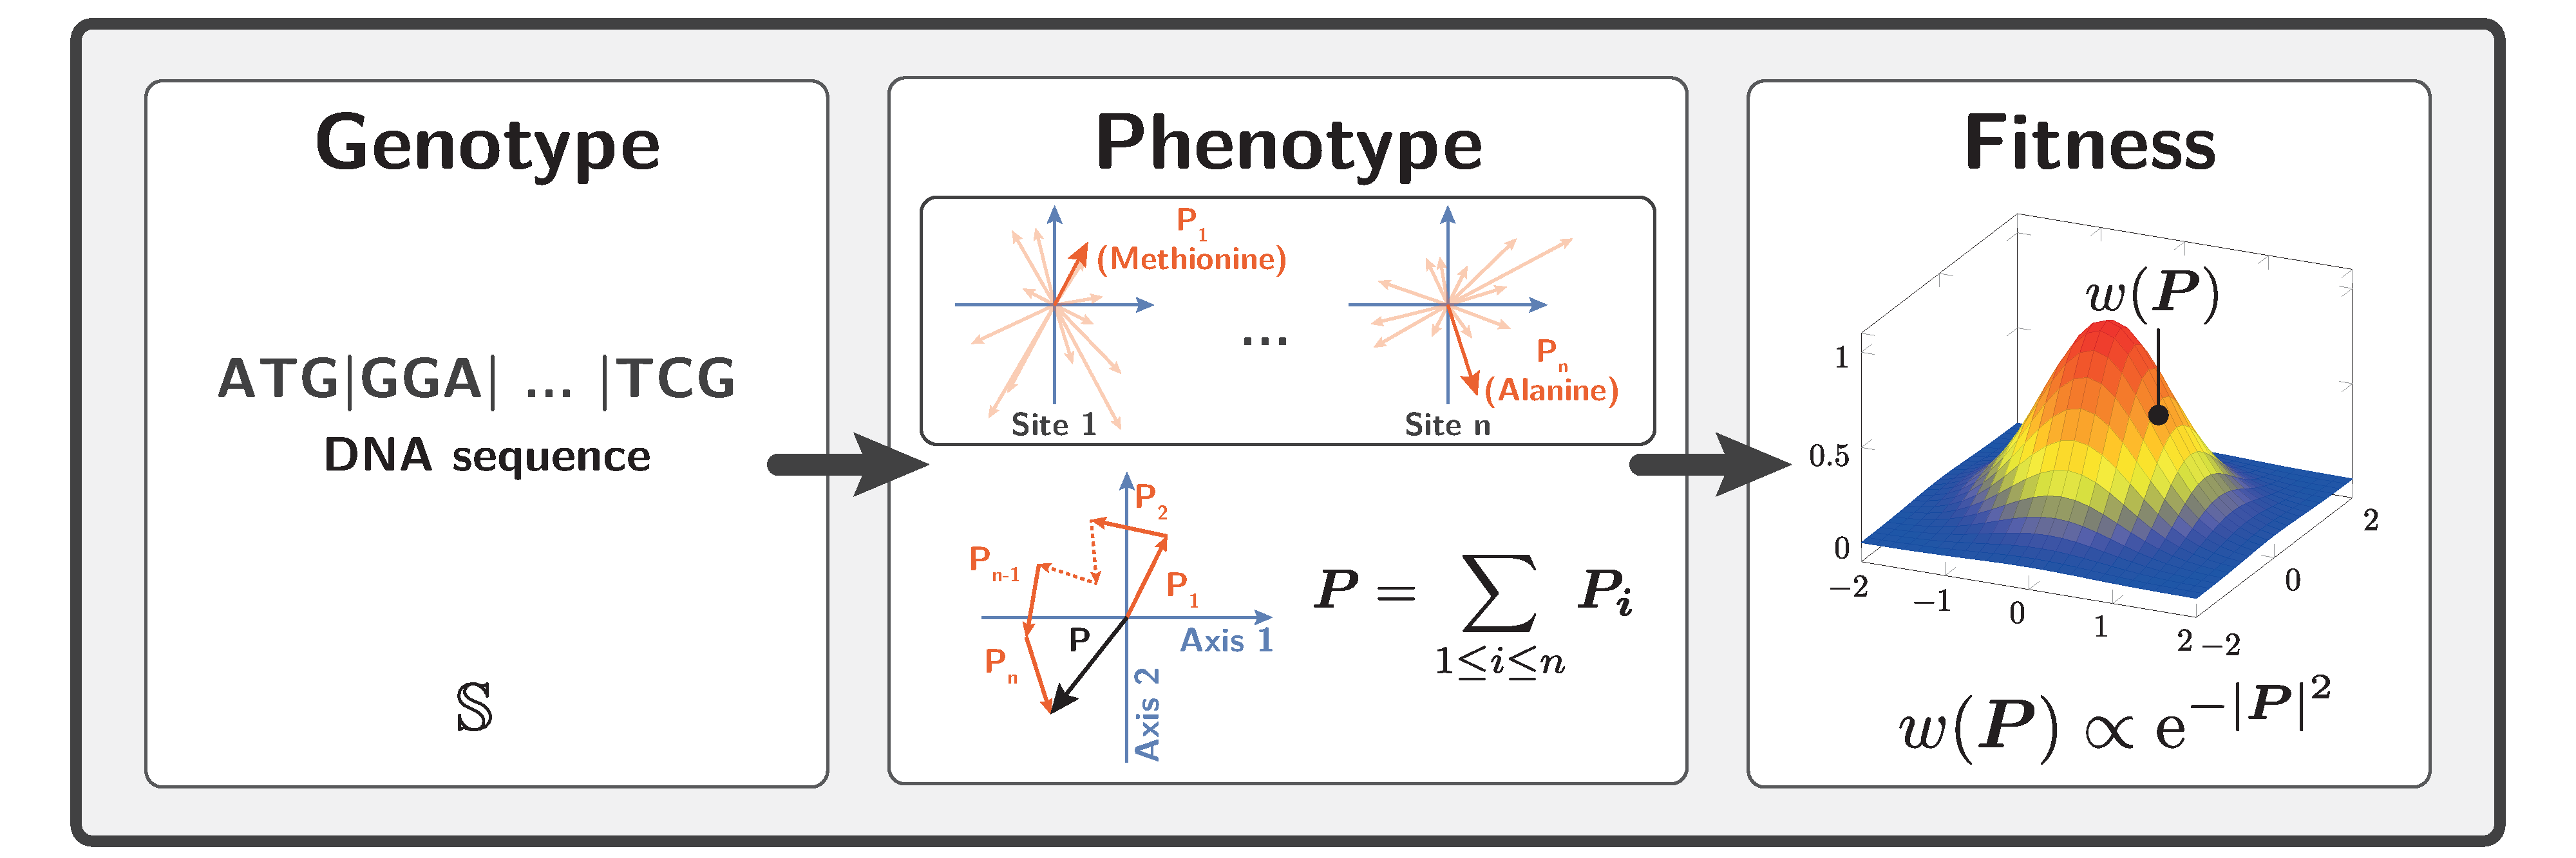
\includegraphics[width=165mm] {artworks/ModelSimuGeo.pdf}
\end{center}
For each possible mutant ($t+1$ substitutions), we compute $\phenoGeo\left(\mathbb{S}^{t+1}\right)$ from the updated sequence $\mathbb{S}^{t+1}$, and subsequently the selection coefficient of the mutant:
\begin{equation}
s \left( \mathbb{S}^{t},\mathbb{S}^{t+1}\right) = \dfrac{ w\left( \phenoGeo\left(\mathbb{S}^{t+1}\right) \right) - w\left( \phenoGeo\left(\mathbb{S}^{t}\right) \right)}{w\left( \phenoGeo\left(\mathbb{S}^{t}\right) \right)}.
\end{equation}
The next change in the protein coding DNA and the time to next the event is chosen using Gillespie algorithm, according to the rates of substitution between codons:
\begin{equation}
{\submatrix_{\itoj}} = \mu_{\itoj} \dfrac{4 \Ne s \left( \mathbb{S}^{t},\mathbb{S}^{t+1}\right)}{{1 - \e^{-4 \Ne \left( \mathbb{S}^{t},\mathbb{S}^{t+1}\right)} }}, 
\end{equation}
where ${\submatrix_{\itoj}} = \mu_{\itoj}$ in the case of synonymous substitutions.

\section{Simulation with protein folding probability}
We simulated substitutions in the protein phosphatase ($\Nsite=300$ codon sites) as in Goldstein \& Pollock (2017).
From a DNA sequence $\mathbb{S}^t$ after $t$ substitutions, we compute the free energy of the folded state $G_{\mathrm{F}}\left(\mathbb{S}^{t}\right)$, using the $3$-dimensional structure of the folded state and pair-wise contact energies between neighboring amino-acid residues:
\begin{equation}
G_{\mathrm{F}}\left(\mathbb{S}^{t}\right) = \sum_{1 \leq \site \leq \Nsite} \sum_{r \in \mathcal{N}(\site)} I \left(\mathbb{S}^t(\site), \mathbb{S}^t(r) \right),
\end{equation}
where $I(a,b)$ is the pair-wise contact energies between amino-acid $a$ and $b$, using contact potentials estimated by Miya-zawa and Jernigan, and $\mathcal{N}(\site)$ are the neighbor residues of site $\site$ (closer than $7\angstrom$) in the $3$D structure.\\

The free energy of unfolded states $G_{\mathrm{U}}\left(\mathbb{S}^{t}\right)$ is approximated using $55$ decoy $3$D structures that supposedly represent a sample of possible unfolded states:
\begin{equation}
G_{\mathrm{U}}\left(\mathbb{S}^{t}\right) = \langle G\left(\mathbb{S}^{t}\right) \rangle - kT \ln (1.0\mathrm{E}^{160}) - \dfrac{2 \left[ \langle G\left(\mathbb{S}^{t}\right)^2 \rangle - \langle G\left(\mathbb{S}^{t}\right) \rangle^2\right] }{kT}
\end{equation}
where the average $\langle . \rangle$ runs other the $55$ decoy $3$D structures, and $k$ is the Boltzmann constant and $T$ the temperature in Kelvin.\\

From the energy of folded and unfolded states, we can compute the difference in free energy between the states:
\begin{equation}
\phenoFold\left(\mathbb{S}^{t}\right) = G_{\mathrm{F}}\left(\mathbb{S}^{t}\right) - G_{\mathrm{U}}\left(\mathbb{S}^{t}\right)
\end{equation}

Wrightian fitness is defined as the probability of our protein to be in the folded state: 
\begin{equation}
w(\phenoFold\left(\mathbb{S}^{t}\right)) = \dfrac{P_{\mathrm{F}}\left(\mathbb{S}^{t}\right)}{P_{\mathrm{F}}\left(\mathbb{S}^{t}\right) + P_{\mathrm{U}}\left(\mathbb{S}^{t}\right)} = \dfrac{e^{-\beta G_{\mathrm{F}}\left(\mathbb{S}^{t}\right) }}{e^{-\beta G_{\mathrm{F}} \left(\mathbb{S}^{t}\right) } + e^{-\beta G_{\mathrm{U}}\left(\mathbb{S}^{t}\right) }} = \dfrac{1}{1 + e^{\beta \phenoFold\left(\mathbb{S}^{t}\right) }}, 
\end{equation}
where $\beta$ is the inverse of the temperature ($\beta=1/kT$).
\begin{center}
	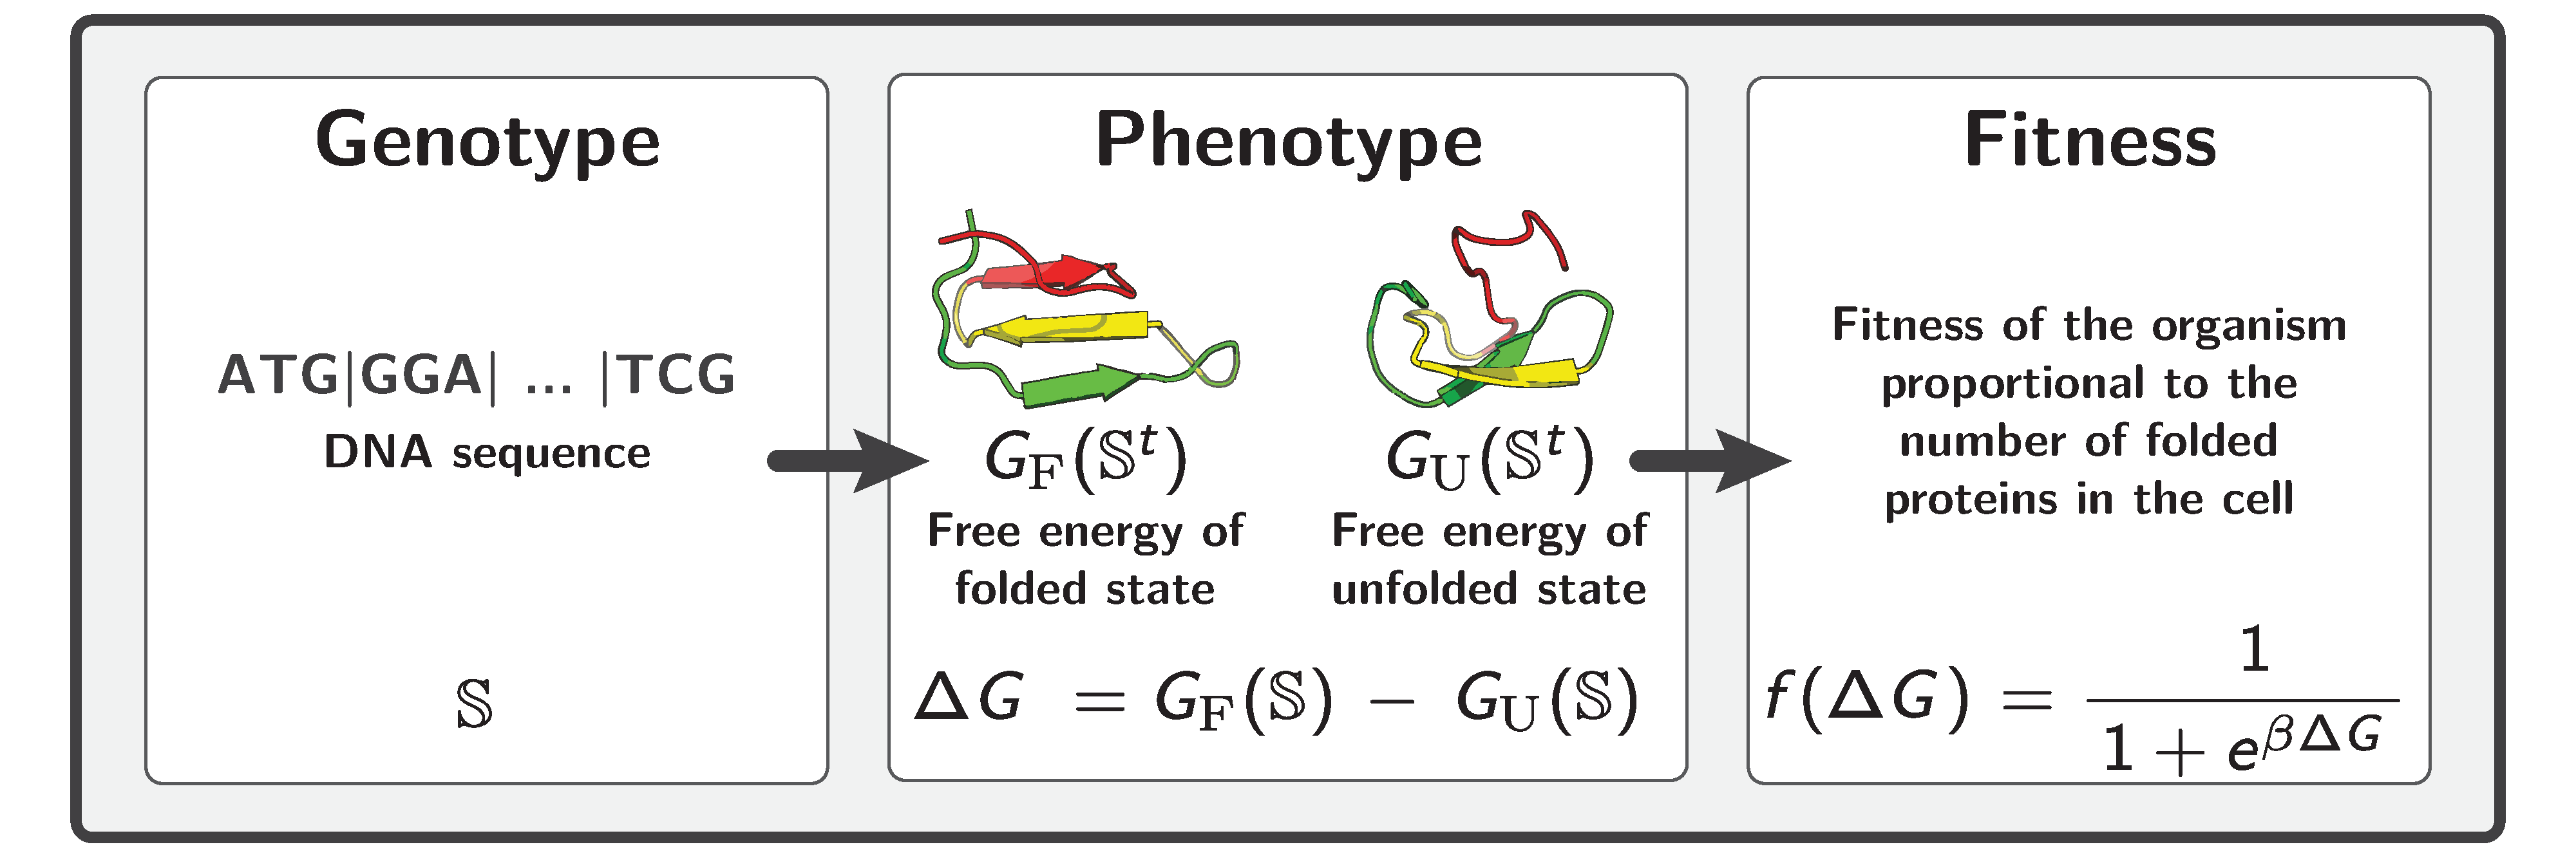
\includegraphics[width=165mm] {artworks/ModelSimuFold.pdf}
\end{center}
For each possible mutant ($t+1$ substitutions), we compute $\phenoFold^{t+1}$ from the updated sequence $\mathbb{S}^{t+1}$, and subsequently the selection coefficient of the mutant:
\begin{equation}
s \left( \mathbb{S}^{t},\mathbb{S}^{t+1}\right) = \dfrac{ w\left( \phenoFold\left(\mathbb{S}^{t+1}\right) \right) - w\left( \phenoFold\left(\mathbb{S}^{t}\right) \right)}{w\left( \phenoFold\left(\mathbb{S}^{t}\right) \right)}.
\end{equation}
The next change in the protein coding DNA and the time to next the event is chosen using Gillespie algorithm, according to the rates of substitution between codons:
\begin{equation}
{\submatrix_{\itoj}} = \mu_{\itoj} \dfrac{4 \Ne s \left( \mathbb{S}^{t},\mathbb{S}^{t+1}\right)}{{1 - \e^{-4 \Ne \left( \mathbb{S}^{t},\mathbb{S}^{t+1}\right)} }}, 
\end{equation}
where ${\submatrix_{\itoj}} = \mu_{\itoj}$ in the case of synonymous substitutions.

\end{document}